\subsection{Análise semanal}
O ponto principal para a escolha ou não da análise semanal é justamente a existência de diferenças das amostras semanais entre si, que justificaria posterior análise dos dados para melhor compreensão\\
\subsubsection{Análise dos tempos de espera e serviço}
O teste não paramétrico de Kolgomorov Smirnov novamente foi utilizado para realização do teste de hipótese.\\
Para que não houvesse uma matriz com as respostas desnecessariamente grande (matriz 52x52) foi realizado o teste apenas para as semanas dos meses de dezembro e janeiro.\\
\begin{center}
    \begin{figure}[H]
        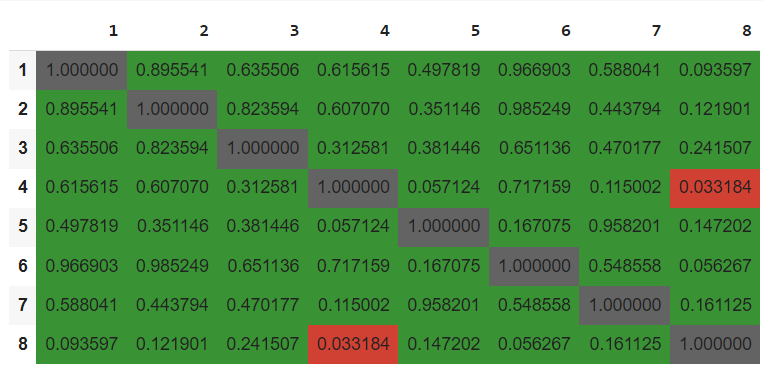
\includegraphics{analise-de-dados/semanal/janas.png}
        \caption{Kolgomorov Smirnov - teste para intervalos de chegada nas semanas de janeiro}
        \label{fig: jan_as_img}
    \end{figure}
    \begin{figure}[H]
        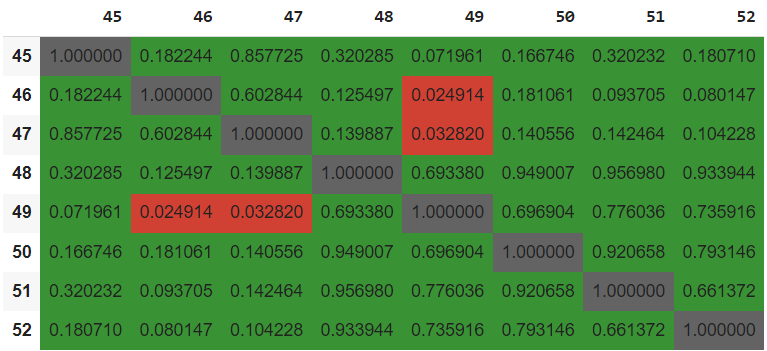
\includegraphics{analise-de-dados/semanal/dezas.png}
        \caption{Kolgomorov Smirnov - teste para intervalos de chegada nas semanas de dezembro}
        \label{fig: dez_as_img}
    \end{figure}
\end{center}
Foi possível observar que no horizonte de planejamento semanal, semanas subsequentes tendem a ter intervalos de chegada que seguem a mesma distribuição de probabilidade e, portanto, o planejamento semanal não é interessante para esse problema, visto que não é possível perceber as diferenças de demanda nesse nível de análise.